\documentclass[twocolumn]{aastex62}

% typography
\usepackage[T1]{fontenc}

\setlength{\parindent}{1.\baselineskip}
\newcommand{\acronym}[1]{{\small{#1}}}
\newcommand{\package}[1]{\textsl{#1}}
\newcommand{\gaia}{\textsl{Gaia}}

% aastex parameters
% \received{not yet; THIS IS A DRAFT}
%\revised{not yet}
%\accepted{not yet}
% % Adds "Submitted to " the arguement.
% \submitjournal{ApJ}
\shorttitle{the jhelum puzzle}
\shortauthors{bonaca et al.}

%@arxiver{}
\usepackage{amsmath}

\begin{document}\sloppy\sloppypar\raggedbottom\frenchspacing % trust me

\title{Multiple components of the cold Jhelum stellar stream}

\correspondingauthor{Ana Bonaca}
\email{ana.bonaca@cfa.harvard.edu}

\author[0000-0002-7846-9787]{Ana Bonaca}
\affil{Center for Astrophysics | Harvard \& Smithsonian, 60 Garden St, Cambridge, MA 02138, USA}

% \author[0000-0002-1590-8551]{Charlie Conroy}
% \affil{Harvard--Smithsonian Center for Astrophysics, 60 Garden St, Cambridge, MA 02138, USA}

\author{collaborators}

% \author[0000-0003-2866-9403]{David W. Hogg}
% \affiliation{Center for Cosmology and Particle Physics,
% Department of Physics,
% New York University}
% \affiliation{Center for Data Science,
% New York University}
% \affiliation{Max-Planck-Institut f\"ur Astronomie, Heidelberg}
% \affiliation{Flatiron Institute, Simons Foundation}

% David, Adrian, Josh, Kathryn

\begin{abstract}\noindent % trust me
- tidally disrupting satellites produce long streams of stars
- until recently, it was only streams from the massive progenitors that have had internal structure
- here we present jhelum -- first cold stream with transverse structure
% Tidally disrupted globular clusters are transformed into thin, dynamically cold streams of stars that are extremely valuable tracers of the large- and small-scale distribution of mass in the Galaxy.
% Using data from the Gaia second data release combined with Pan-STARRS photometry, we present a sample of highly probable members of the longest cold stream in the Milky Way, GD-1.
% The resulting map of GD-1: (1) extends the apparent length of the stream by 20, (2) reveals plausible locations for the progenitor, (3) detects high-contrast gaps along the stream, and (4) indicates the existence of stream members perturbed off the main stream track.
% These discoveries are only possible because of the exquisite astrometry from Gaia, which permits a clean separation of the stream from Milky Way stars.
% The additional length and a proper treatment of the progenitor will aid in dynamical modeling of GD-1 for mapping the large-scale dark matter distribution.
% The complex morphology of the stream points to a turbulent history; detailed phase-space properties of the perturbed stream members could potentially constrain dark matter substructure in the Milky Way.
\end{abstract}

\keywords{%
stars:~kinematics~and~dynamics
  ---
Galaxy:~halo
  ---
Galaxy:~kinematics~and~dynamics
}

\section{Introduction}
\label{sec:intro}

- mw provides opportunity to study processes of gal formation in archaelogical evidence
- halo dynamical times, streams track that change

- streams regular so far
- dynamical environment, should have features
- now with gaia can study those

Stars escaping from globular clusters form thin, dynamically cold tidal streams \citep[e.g.,][]{combes1999}.
The phase-space distribution of tidal debris is predominantly determined by the gravitational tidal field, so \citet{johnston1999} proposed measuring the distribution of matter in the Galaxy using stellar streams.
In detail, the mean track of a stream constrains the enclosed mass at its current location \citep{bh2018}.
As more than 40 stellar streams have been discovered at a range of distances in the Milky Way halo \citep[see][for a recent review]{gc2016}, streams should provide a three-dimensional map of the Galaxy.

Being long and thin structures, stellar streams also preserve a historical record of gravitational perturbations on small scales and have been discussed as tracers of dark matter substructure \citep[e.g.,][]{johnston2002, carlberg2009}.
A telltale signature of an interaction with a dark matter subhalo is a gap in the stellar density along the stream \citep[e.g.,][]{yoon2011, eb2015}.
Tantalizing hints of stream gaps were first observed in the early photometric surveys \citep[e.g.,][]{carlberg2012,cg2013}, and gaps were definitively detected in the GD-1 stellar stream \citep{gd2006} when \citet{pwb} used \gaia\ proper motions to cleanly select likely stream members.
This discovery opened a new era in which globular cluster streams are no longer simple tracers of the global gravitational potential, but instead provide additional constraints  through their complex density structure.

In addition to opening gaps along the stream, a dynamic, clumpy and/or time-dependent, environment can disperse stars from originally thin streams to form much wider structures \citep[e.g.,][]{bonaca2014, ngan2016, pw2016, pearson2017}.
Alternatively, a globular cluster that started disrupting in a satellite galaxy before its accretion to the main Milky Way halo, creates a cold stream that is also accompanied by a wide, low surface-brightness component (Carlberg, in preparation).
Wide extensions have not yet been detected around the known cold streams, however, recent improvements in identifying stream members motivate a more comprehensive search.

Here we present the first evidence for two components of the Jhelum stream.
Discovered as a photometric overdensity in the Dark Energy Survey \citep[DES,][]{abbott2018}, Jhelum is a $\sim30^\circ$ long and $\sim1^\circ$ wide stellar stream at a distance of $\sim13\,$kpc \citep{shipp2018}.
Like GD-1, Jhelum is also on a retrograde orbit with respect to the Milky Way disk \citep{malhan2018}, so we use \gaia\ proper motions in addition to DES photometry to better select likely members (\S\ref{sec:data}).
The resulting map of the stream reveals that Jhelum has a thin and a wide component; we compare and contrast these components in \S\ref{sec:structure}.
In \S\ref{sec:discussion} we conclude with a discussion of possible origin scenarios.

% - streams expected to trace the gravitational potential
% - cold streams optimal because simple structures, easy to model
% 
% - cold streams so far indeed looked regular
% - very similar N-body models of disrupting globular clusters in simple potentials
% - however, in more realistic (live, nbody) potential they are often disturbed
% 
% - from photometric data alone, tenative signs of disturbance are present in the closest stream -- GD-1
% - these were made certain with Gaia selection -- evidence not only of gaps, but also of extra stream material
% - suggests that further scrutiny of Galactic streams is warranted, as they might not be as simple as previously thought


\section{Data}
\label{sec:data}
We start our analysis by defining a coordinate system $(\phi_1,\phi_2)$ that is aligned with the Jhelum stellar stream.
The great circle best-fitting the Jhelum track has a pole $(\alpha_{2000},\delta_{2000}) = (359.1^\circ, 38.2^\circ)$ \citep{shipp2018}.
The rotation matrix\footnote{Also available electronically at \url{https://github.com/abonaca/jhelum}.} that converts equatorial $(\alpha, \delta)$ coordinates to Jhelum coordinates $(\phi_1, \phi_2)$, where $\phi_1$ is the coordinate along the stream and $\phi_2$ is perpendicular to the stream track, is provided in the Appendix.
In these coordinates, Jhelum is centered at $\phi_2=0$, and the DES detection spans $-5^\circ\lesssim\phi_1\lesssim25^\circ$ \citep{shipp2018}.

\begin{figure}
\begin{center}
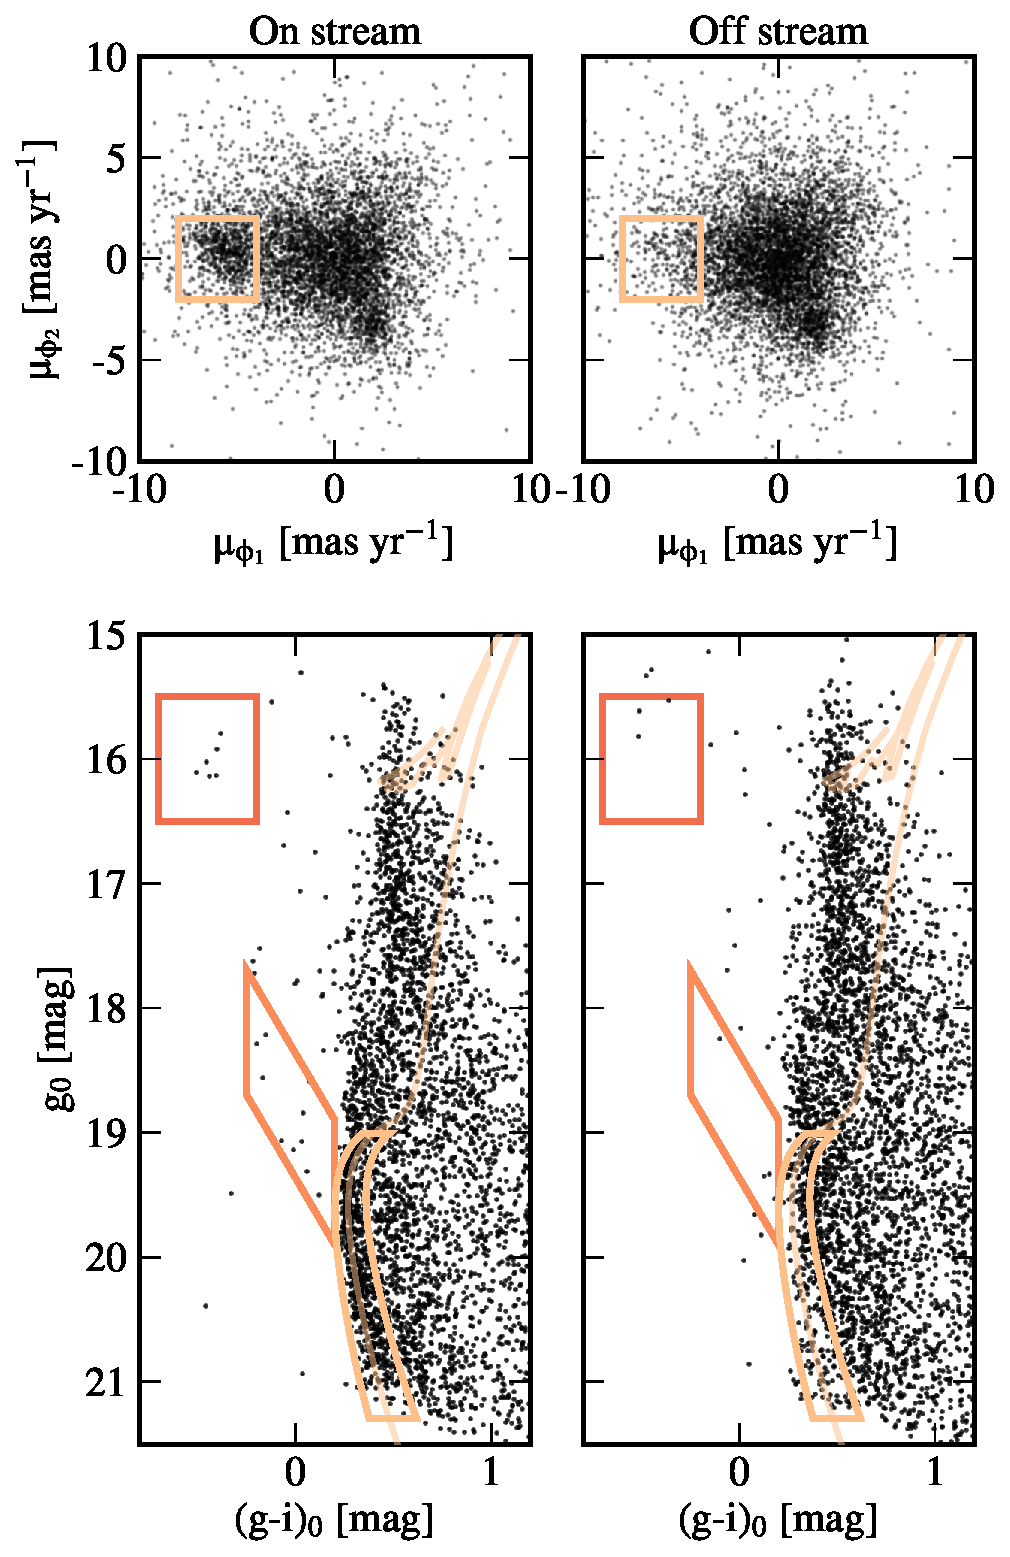
\includegraphics[width=0.95\columnwidth]{selection.pdf}
\end{center}
\caption{
(Top) Proper motions of photometry-selected stars along the Jhelum stream (left) and in a control field (right). 
(Bottom) Similarly, color-magnitude diagrams of stars selected on proper motions.
Photometric and proper-motion selection boxes are shown in light orange.
Jhelum stands out from the Milky Way field population in proper motions as a retrograde stream, and in the color-magnitude diagram where its main sequence is more metal-poor than the field, and is accompanied by blue stragglers (medium orange) and blue horizontal branch stars (dark orange box).
}
\label{fig:properties}
\end{figure}

We query the Gaia DR2 \citep{gdr2} and DES DR1 \citep{abbott2018} catalogs between $-10^\circ<\phi_1<35^\circ$ and $-5^\circ<\phi_2<5^\circ$, and select all sources identified as stars that are brighter than $g_0<23$, while excluding stars with parallaxes larger than $1\,\rm mas$.
DES photometry was dereddened using \citet{sfd} dust maps.
Assuming a constant distance along the stream of 13\,kpc, we correct the whole catalog for the solar reflex motion following \citet{pwb}.

Following these corrections, Jhelum stars becomes readily distinct from the Milky Way field population.
Figure~\ref{fig:properties} shows proper motions (top) and color-magnitude diagram (bottom) for a stream field ($0^\circ<\phi_1<25^\circ$, $0^\circ<\phi_2<1^\circ$, left) and a comparison field ($0^\circ<\phi_1<25^\circ$, $3.5^\circ<|\phi_2|<4^\circ$, right).
In proper motions, Jhelum stands out from the Milky Way as a retrograde stream, and we select likely members between $-8<\mu_{\phi_1,\star}/{\rm mas\,yr^{-1}}<-4$ and $-2<\mu_{\phi_2}/{\rm mas\,yr^{-1}}<2$.
The stream also appears as a prominent overdensity of main sequence stars, which we select following a 12\,Gyr old, metal-poor ($\rm[Fe/H]=-1.5$) MIST isochrone \citep{choi2016} between $19<g_0<21.3$.
Both of these selection regions are shown in light orange in Figure~\ref{fig:properties}.
In the next section, we discuss the spatial distribution of identified Jhelum member stars.


\section{Density structure of Jhelum}
\label{sec:structure}

\begin{figure*}
\begin{center}
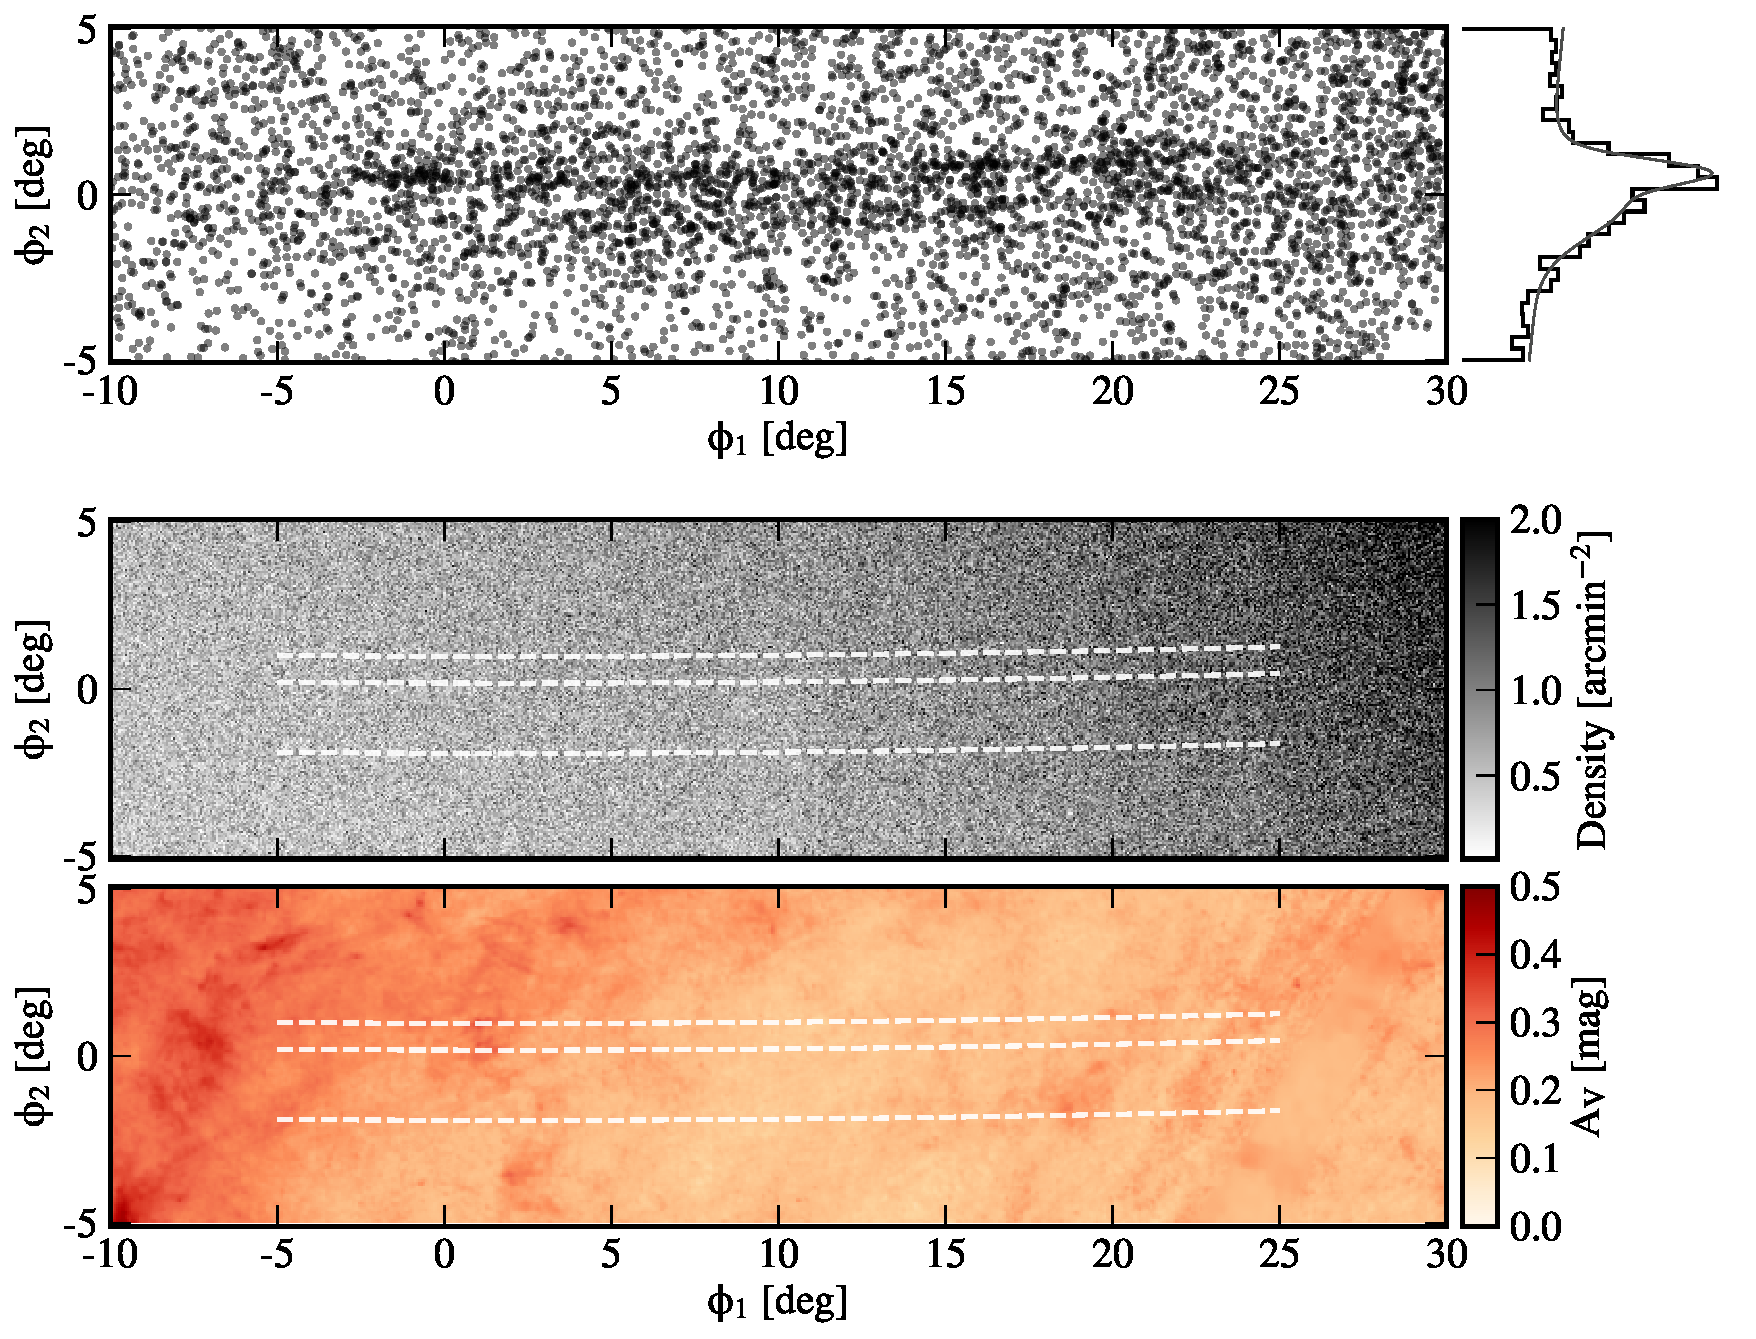
\includegraphics[width=0.9\textwidth]{map.pdf}
\end{center}
\caption{
(Top left) Sky positions of likely Jhelum members in the stream coordinate system reveal for the first time a complex morphology in a cold stream.
Member selection is based on the \gaia\ proper motions and DES photometry, and excludes nearby contaminants using \gaia\ parallaxes.
(Top right) Profile of likely Jhelum members between $-5^\circ<\phi_1<25^\circ$ is asymmetric, with a narrow, dense component at $\phi_2>0^\circ$ and a more diffuse, wide component at $\phi_2<0^\circ$.
This morphology is intrinsic to the stellar stream, as similar signatures are absent from the full stellar density field (middle) and the dust map (bottom).
}
\label{fig:map}
\end{figure*}

Sky positions of Jhelum members selected in Section~\ref{sec:data} are presented in the top left panel of Figure~\ref{fig:map}. 
Although some contamination from the Milky Way field stars remains, the stream stands out as an overdensity between $-5^\circ<\phi_1<25^\circ$, $-1^\circ<\phi_2<1^\circ$.
Despite the increase in the purity of the stream membership, this extent is similar to the initial detection reported by \citet{shipp2018}.
However, the new data reveal unexpected internal structure of the stream: the density of stream members is higher at $\phi_2>0$ than at $\phi_2<0$.
The $\phi_2$ distribution of likely Jhelum members (Figure~\ref{fig:map}, top right) appears bimodal, with a more prominent, narrow component at $\phi_2>0$, and a less prominent, diffuse component peaking at $\phi_2\approx0$.

Surveys such as Gaia and DES have complex selection functions \citep[e.g.,][]{bovy2017}, which can imprint density inhomogeneities in all stellar maps.
To test whether the density structure observed in Jhelum is inherited from a survey strategy, we show a density map of all stars in our input catalog (Gaia crossmatched with DES, and with parallax $\varpi<1\,\rm mas$) in the middle panel of Figure~\ref{fig:map}.
Dashed white lines bracket the two Jhelum components.
The lines are offset from the best-fitting polynomial to the running median of the dense Jhelum component: $\phi_2 = 0.000546 \,\phi_1^2 -0.00217 \,\phi_1 +0.583$.
Whereas there is a large density gradient along the $\phi_1$ direction, as positive $\phi_1$ values correspond to lower galactic latitudes, the overall stellar density changes little across the stream in the $\phi_2$ direction at a fixed $\phi_1$ location.

Density variations observed in streams can also originate from nonuniform dust attenuation \citep[e.g.,][]{ibata2016}.
In that case, the features observed in the stream correlate with a dust map.
Extinction along Jhelum varies between $A_V\sim0.2-0.5$ \citep[Figure~\ref{fig:map}, bottom;][]{sfd}.
The regions of high dust attenuation at $(\phi_1,\phi_2)\approx(1^\circ,0.5^\circ)$ and $(\phi_1,\phi_2)\approx(19^\circ,-2^\circ)$ correspond to regions of reduced Jhelum density, however, there are no global gradients in dust extinction perpendicular to the stream.
Therefore, the transverse variations in Jhelum density are intrinsic to the stream itself.

\begin{figure*}
\begin{center}
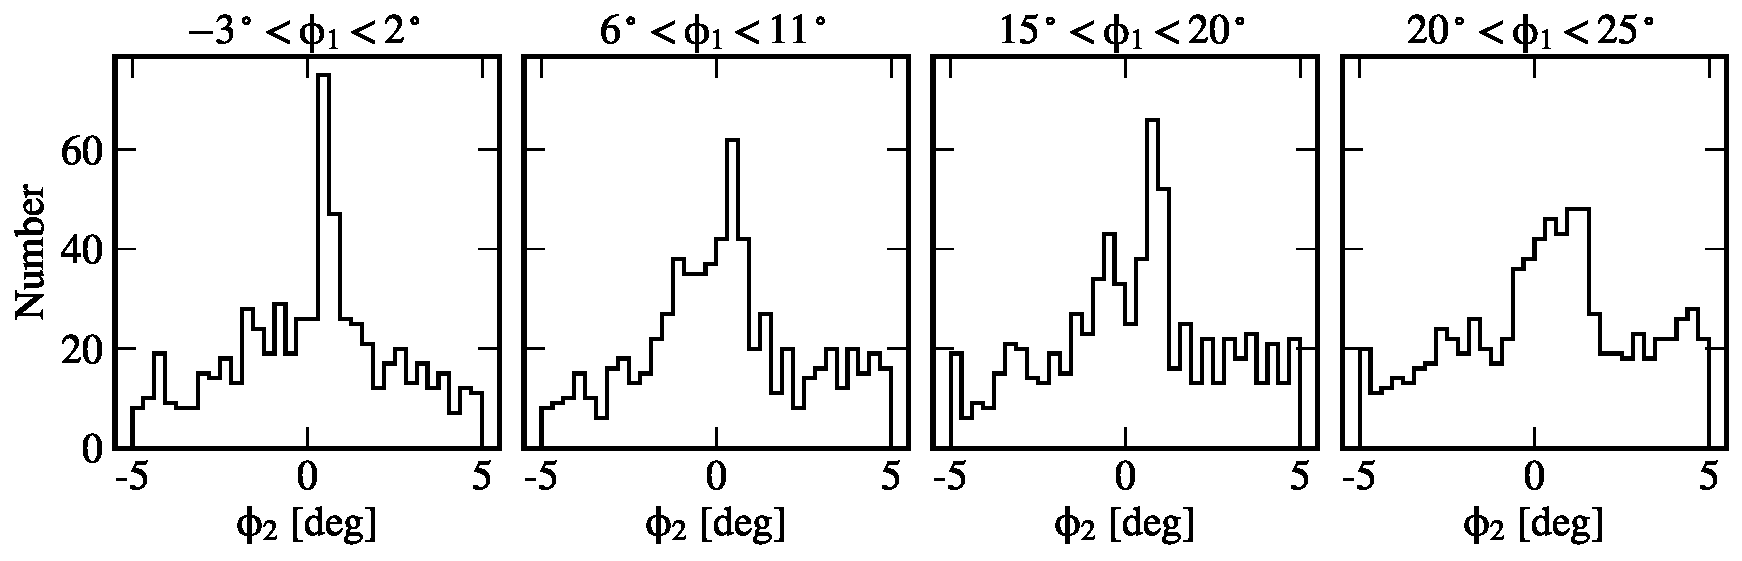
\includegraphics[width=0.9\textwidth]{phi2_histograms.pdf}
\end{center}
\caption{
Histograms
}
\label{fig:histo}
\end{figure*}

- two component fit is better than a single component
- significance / properties of the two components change along the stream 


\section{The origin of Jhelum components}
\label{sec:origin}
- for simplicity, we consider just two components
- first branch: multiple / single progenitor

- bhb / bs, not common in the field
- absolute value consistent with both gc \& dwarfs
- ratio the same in the two components
- points to a single progenitor, but detailed abundances necessary to confirm 

\begin{figure*}
\begin{center}
\includegraphics[width=0.7\textwidth]{orbit_galactocentric.pdf}
\end{center}
\caption{
Best-fitting orbit of the Jhelum stellar stream in the disk plane (left) and perpendicular to the plane (right).
Thicker portion of the line denotes the observed extent of the stream, while the insets present likely Jhelum members in these coordinates.
}
\label{fig:galactocentric}
\end{figure*}

- if indeed a single progenitor, could be that just projected 2 component, but in fact a sheet whose one side is observed edge-on in a fold 
- if such a shell, would expect the denser part to be at the apocenter
- to test this, we need distances
- parallaxes bad, but bhb standard candles, no difference, no gradient
- photometric distances, same conclusion
- assuming distance constant and 13\,kpc, the likely members in cylindrical coordinates on figure
- denser part at the inner z edge -- not a conventional shell / fold

% then a dynamical process shaped it, either before the full disruption (e.g., substructure in the progenitor) or after (e.g., something in the global potential), e.g., caustic
- external perturbations have been shown to affect streams, such as the lmc or the bar
- to assess, we find a best fitting orbit to the narrow track, bhb for distances, proper motions
- assuming a simple multi-component MW potential

% - goodness of fit
% - predictions for radial velocity
% - model on this orbit is a good fit to the track, but a single component

- best-fitting orbit is regular, chaos not important on relevant time scales (lyapunov time)
- inner halo -- not lmc, but might be influenced by the bar
- this is not very likely as the stream is retrograde, but merits further investigation
% - orbital period, distance -- corrotation with the bar? although retrograde..

% - no multiple wraps along the wide component
% - if an older wrap, question of where is the rest of the stream, ie why just 30deg long
% - some additional effect missing, we discuss the options below

\section{Discussion}
\label{sec:discussion}
- summary
- same progenitor, truly 2 components, not reproducible in a simple static model

- listing of possible other explanations:
\begin{itemize}
 \item multiple progenitors (e.g., gc + dwarf galaxy) -- however, stellar populations uniform across the stream, but could further test with chemical abundances
 \item dynamically cold structure in the progenitor -- contrived?
 \item caustic -- would happen preferentially at the apocenter, but stream is just past the pericenter, so this type ruled out, however, it could be also a caustic of a fully phase-mixed distribution
 \item chaos -- would need to be close to a resonant orbit, but orbit looks regular (although chaotic orbit might still be possible if the adopted potential is very different from the true one)
 \item precession of orbital plane if close to the disk on approx circular orbit (Dehnen2018), or if pericenter is close to the center of the Galaxy (eccentric orbit at some angle wrt the disk; Erkal2016) -- eccentricity = 0.5, zmax = 30 kpc; -- not captured in the streakline model
%  \item lmc effect? -- not that close in the past
%  \item a bar effect? -- seems like crossed the plane at very small x, y ($R\sim7\,\rm kpc$), will create a stream model in a barred potential
\end{itemize}

- multiple wraps -- globular clusters disrupting in a cosmological N-body dark matter halo produce cold streams that are accompanied by a diffuse, dynamically older component (R.~Carlberg, private communication), penarrubia

- spectroscopy will help -- test single progenitor through chemical abundances
- can distinguish between different scenarios based on mean radial velocity trends and also velocity dispersion

- rich in information


\appendix
% \section{Jhelum rotation matrix}
% \begin{widetext}
\begin{equation*}
\begin{bmatrix}
\cos(\phi_1)\cos(\phi_2)\\
\sin(\phi_1)\cos(\phi_2)\\
\sin(\phi_2)\\
\end{bmatrix}
 = 
\begin{bmatrix}
0.6173151074 & -0.0093826715 & -0.7866600433 \\ 
-0.0151801852 & -0.9998847743 & 0.0000135163 \\ 
-0.7865695266 & 0.0119333013 & -0.6173864075 \\ 

\end{bmatrix}
\begin{bmatrix}
\cos(\alpha)\cos(\delta)\\
\sin(\alpha)\cos(\delta)\\
\sin(\delta)\\
\end{bmatrix}
\label{eq:rotmat}
\end{equation*}
% \end{widetext}

\bibliographystyle{aasjournal}
\bibliography{jhelum}



\end{document}

